\documentclass[14pt, a4paper]{report}
\usepackage{mathtext}
\usepackage[T2A]{fontenc}
\usepackage[utf8]{inputenc}
\usepackage[russian]{babel}
\usepackage{multirow}
\usepackage{slashbox}
\usepackage{makecell}
\usepackage{graphicx}
\usepackage{physics}
\usepackage{amstext}
\usepackage{caption}
\usepackage{subcaption}
\usepackage{cmap}
\usepackage{float}
\usepackage{indentfirst}
\usepackage{romannum}

\usepackage[a4paper,
            		left=1in,
            		right=1in,
           		 top=1in,
            		bottom=1in,
            		footskip=.25in]{geometry}

\renewcommand{\thesection}{\arabic{section}.}
\renewcommand{\thesubsection}{\arabic{section}.\arabic{subsection}.}

\title{\textbf{Отчет о выполнении лабораторной работы 1.3 "Эффект Рамзауэра"}}
\author{Калашников Михаил, Б03-202}
\date{}

\begin{document}
\maketitle

\textbf{Цель работы:}
Исследование энергетической зависимости вероятности рассеяния электронов атомами ксенона, определение энергии электронов, при которых наблюдается "просветление" ксенона, и оценивание размера его внешней электронной оболочки.
\newline

\section{Теоретические сведения}

Эффективным сечением реакции называется величина, характеризующая вероятность перехода системы двух сталкивающихся частиц в результате их рассеяния в определенное конечное состояние. Сечение $\sigma$ равно отношению числа $N$ таких переходов в единицу времени к плотности $nv$ потока рассеиваемых частиц.

\[\sigma=\frac{N}{nv}\]

\begin{figure}[H]
\centering
\begin{minipage}{.5\textwidth}
  \centering
  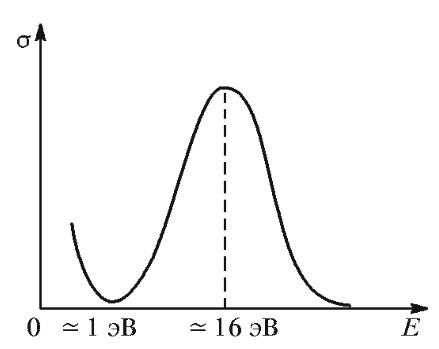
\includegraphics[width=.8\linewidth]{../images/513-1}
  \caption{Качественная картина результатов измерения упругого рассеяния электронов в аргоне}
\end{minipage}%
\begin{minipage}{.5\textwidth}
  \centering
  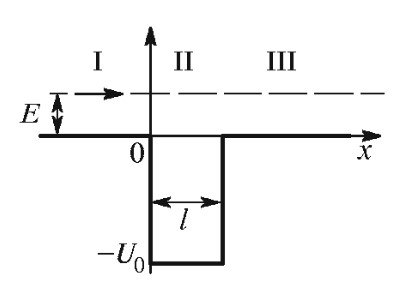
\includegraphics[width=.8\linewidth]{../images/513-2}
  \caption{Схематическое изображение прямоугольной потенциальной ямы, над которой пролетаем частица с энергией E}
\end{minipage}
\end{figure}

Объяснение эффекта, приведенного на рисунке выше, требует учета волновой природы электронов. Рассмотрим электрон, проходящий через плоскую прямоугольную потенциальную яму шириной $l$ и глубиной $U_0$. Уравнение Шредингера в данном случае примет вид:

\begin{equation}[H]
	\psi``+k^2\psi=0,\quad где\ k^2=
 	\begin{cases}
	k_1^2=\frac{2mE}{\hbar^2} \text{ -- в областях \Romannum{1} и \Romannum{3};}\\
	k_2^2=\frac{2m(E+U_0)}{\hbar^2} \text{ -- в области \Romannum{2}.}
	\end{cases}
\end{equation}

Коэффициент прохождения $D$ при этом равен отношению квадратов амплитуд прошедшей и падающей волн:

\[D^{-1}=1+\frac{U_0^2}{4E(E+U_0)}\sin^2{k_2l}\text{.}\]

Коэффициент прохождения максимален при условии:

\[k_2l=\sqrt{\frac{2m(E + U_0)}{\hbar^2}}l=n\pi,\quad n=1,2,3...\text{.}\]

Рассмотрим интерференцию электронных волн де Бройля в атоме. Прошедшая волна усилится дважды отраженной при условии $\Delta=2l=\lambda`$. С другой стороны, прошедшая волна ослабится если $\Delta=2l=(3/2)\lambda`$. Получим два уравнения:

\[2l=\frac{h}{\sqrt{2m(E_1+U_0)}}\text{,}\quad 2l=\frac{3}{2}\frac{h}{\sqrt{2m(E_2+U_0)}}\text{.}\]

Решая эти два уравнения можно найти эффективный размер атома $l$ и эффективную глубину потенциальной ямы атома:

\[l=\sqrt{h\sqrt{5}}{\sqrt{32m(E_2-E_1)}}\text{,}\quad U_0=\frac{4}{5}E_2-\frac{9}{5}E_1\text{.}\]

\section{Экспериментальная установка}

Для изучения эффекта Рамзауэра используется тиратон ТГ3-01/1.3Б, заполненный инертным газом.

\begin{figure}[H]
\centering
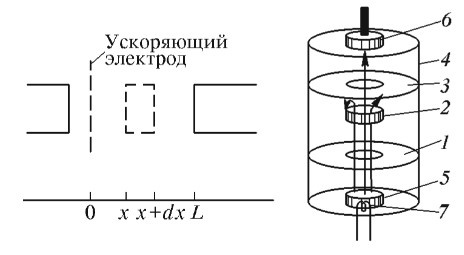
\includegraphics[scale=0.8]{../images/513-3}
\caption{Схематическое изображение тиратона (слева) и его конструкция (справа): 1, 2, 3 -- сетки; 4 -- внешний металлический цилиндр; 5 -- катод; 6 -- анод; 7 -- накаливаемая спираль}
\end{figure}

Электроны, эмитируемые катодом тиратона, ускоряются напряжением V, приложенным между катодом и ближайшей к нему сеткой. Затем электроны рассеиваются на атомах ксенона.

\section{Проведение эксперимента}

\section{Обработка результатов}

\section{Выводы}

\end{document}